\chapter{Multi Body Dynamics Vehicle Model with a Towing Winch}\label{ch:RMBDW}

In this chapter, a multi-body dynamics model of a MT865 tractor equipped with a hydraulic towing winch will be derived where only longitudinal motion is considered. The reason for this restriction is twofold. First this greatly simplifies the governing differential equations. Second, the mechanics and dynamics of tracked vehicles cause turning vehicle trajectories to significantly decrease traction. There is a similar traverse in Greenland called the Greenland Inland Traverse (GrIT) that already uses a winch. A picture of this is shown in Fig. \ref{fig:GrIT_CASE_Tractors} to illustrate its implementation where the winch is mounted at the rear of the vehicle. 
\begin{figure}[b]
\centering
\begin{subfigure}{0.6\textwidth}
\centering
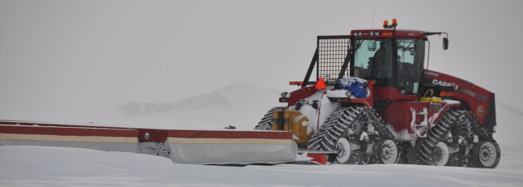
\includegraphics[height = 3.3 cm, keepaspectratio]{CASE_Winch_Full_Tractor}
\caption{}
\label{fig:CASE_Winch_Full_Tractor}
\end{subfigure}
\begin{subfigure}{0.3\textwidth}
\centering
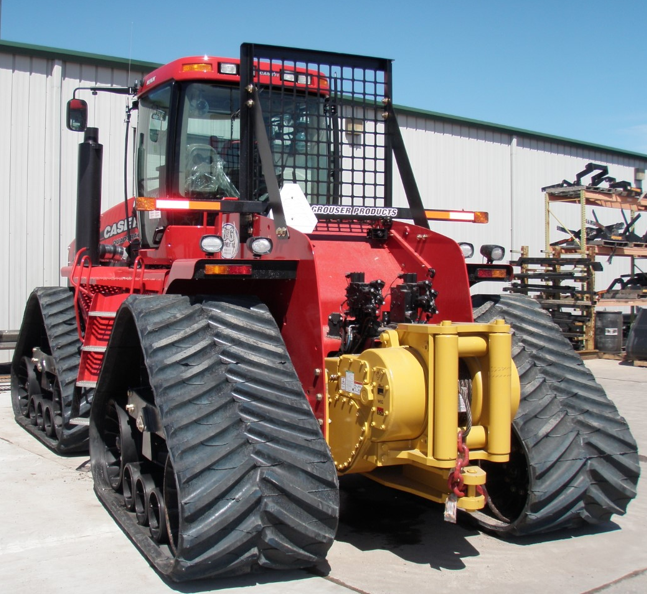
\includegraphics[height = 3.3cm, keepaspectratio]{CASE_WINCH_PICTURE_NO_SLED}
\caption{}
\label{fig:CASE_WINCH_PICTURE_NO_SLED}
\end{subfigure}
\caption{Two pictures of a GrIT Case Quadtrac tractor equipped with a hydraulic towing winch. (a) Right, rear view of GrIT tractor equipped with a towing winch and sled. (b) Rear view of a GrIT tractor equipped with only a towing winch showing implement valve connections and winch cable}
\label{fig:GrIT_CASE_Tractors}
\end{figure}
This multi-body winch model will be used to test the viability of approaches for control mode 3. In this model derivation, actuator limitations are captured as physically motivated models for the hydraulic components are used and put additional load on the tractor's engine under operation. The winch cable is assumed to be a rigid body only capable of holding loads in tension. Modeling of more complex cable towing systems have been investigated for marine vehicles where one vehicle tows another \cite{sanders1982three,kamman2001multibody,kamman1999modeling,milinazzo1987efficient}. In these studies, the path of the towed vehicle is the control variable of interest. Therefore, knowing the cable’s position and trajectory along its entire length is essential for the desired control performance. Modeling of the cable includes finite-segment, rigid link lumped parameter elements that include fluid dynamics. The objective of interest motivating the modeling presented in this chapter is mobility of the towing vehicle. This justifies the use of a simpler approach to account for cable dynamics. 

\import{Chapter4/}{Newton_Euler_Model_Derivation}
\import{Chapter4/}{Winch_Hydraulics}
\import{Chapter4/}{Hybrid_Dynamics_and_Event_Detection}
\import{Chapter4/}{Simulation_Results}